\section{Příklad 1}
% Jako parametr zadejte skupinu (A-H)
\prvniZadani{A}

\subsection{Řešení}

Naším úkolem je vypočítat napětí a proud rezistoru $R_2$. Jako první pomocí postupných záměn 
zjistíme celkový ekvivalentní odpor obvodu $R_e$. Jako první nahradíme sériově zapojené 
rezistory $R_6$ a $R_8$ ekvivalentním odporem $R_{68}$ o velikosti:

$$ R_{68} = R_6 + R_8 = 940 \Omega$$

\begin{figure}[H]
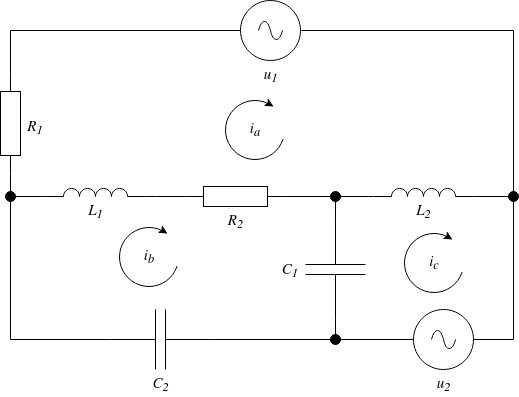
\includegraphics[scale=0.5]{Pr1/step1.png}
\centering
\caption{Odpor $R_{68}$}
\end{figure}

Následně si označíme uzly $A$, $B$, $C$ (viz předchozí obrázek), a zaměníme trojúhelník tvořený rezistory $R_5$, $R_7$ a $R_{68}$ hvězdou s ekvivalentními odpory $R_a$, $R_b$, a $R_c$. Jejich velikosti vypočítáme pomocí následujících vztahů:

$$ R_a = \frac{R_5R_{68}}{R_5 + R_7 + R_{68}} \doteq 210,1863 \Omega$$
$$ R_b = \frac{R_5R_7}{R_5 + R_7 + R_{68}} \doteq 69,3168 \Omega$$
$$ R_c = \frac{R_7R_{68}}{R_5 + R_7 + R_{68}} \doteq 180,9938 \Omega$$

\begin{figure}[H]
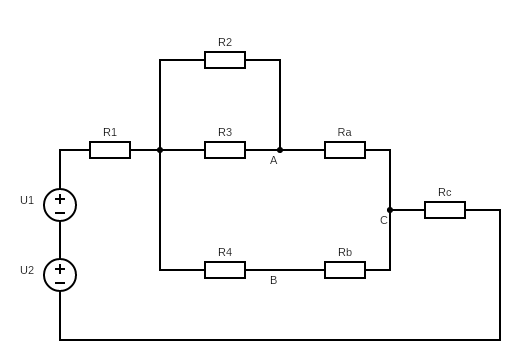
\includegraphics[scale=0.5]{Pr1/step2.png}
\centering
\caption{Záměna hvězdy za čtverec}
\end{figure}

Nyní nahradíme paralelně zapojené rezistory $R_2$ a $R_3$ ekv. odporem $R_{23}$ a sériově zapojené odpory $R_4$ a $R_b$ odporem $R_{4b}$:

$$ R_{23} = \frac{R_2R_3}{R_3 + R_3} \doteq 251,4151 \Omega $$
$$ R_{4b} = R_4 + R_b = 199,3168 \Omega $$

\begin{figure}[H]
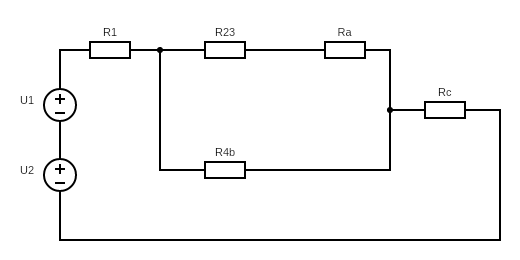
\includegraphics[scale=0.5]{Pr1/step3.png}
\centering
\caption{Odpory $R_{23}$ a $R_{4b}$}
\end{figure}

Následně můžeme nahradit pár sériově zapojených odporů $R_{23}$ a $R_a$ jedním odporem $R_{23a}$:

$$ R_{23a} = R_{23} + R_a = 461,6014 \Omega $$

\begin{figure}[H]
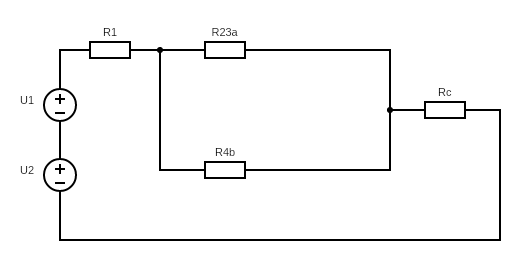
\includegraphics[scale=0.5]{Pr1/step4.png}
\centering
\caption{Odpory $R_{23}$ a $R_{4b}$}
\end{figure}

Dále nahradíme paralelně zapojené $R_{23a}$ a $R_{4b}$ odporem $R_d$:

$$ R_d = \frac{R_{23a}R_{4b}}{R_{23a} + R_{4b}} \doteq 141,9836 \Omega $$

\begin{figure}[H]
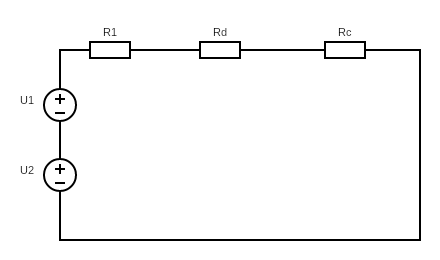
\includegraphics[scale=0.5]{Pr1/step5.png}
\centering
\caption{Odpor $R_d$}
\end{figure}

Nakonec nahradíme tři sériově zapojené odpory $R_1$, $R_d$ a $R_c$ ekvivalentním odporem celého 
obvodu $R_e$, a sériově zapojené napěťové zdroje $U_1$ a $U_2$ ekvivalentním zdrojem $U_{12}$:

$$ R_e = R_1 + R_d + R_c = 141,9836 \Omega $$
$$ U_{12} = U_1 + U_2 = 200 V $$

\begin{figure}[H]
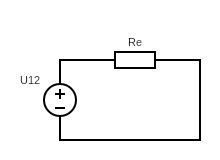
\includegraphics[scale=0.5]{Pr1/final.png}
\centering
\caption{Zjednodušený obvod}
\end{figure}

Když už známe celkový odpor rezistorů a celkové napětí zdrojů v obvodu, můžeme dle Ohmova zákona spočítat 
proud $I_e$ procházející rezistorem $R_e$:

$$ I_e = \frac{U_{12}}{R_e} \doteq 0,2984 A $$ 

Proud $I_d$ procházející odporem $R_d$ je stejný jako proud $I_e$, jelikož rezistory z obr. 5 jsou zapojeny v 
sérii. Tento proud se dle prvního Kirchoffova zákona rozdělí do větví s odpory $R_{23a}$ a $R_{4b}$.
$$ I_d = I_{23a} + I_{4b} $$
Napětí na rezistoru $R_{23a}$ je stejné jako napětí na $R_d$, viz obr. 5. $U_d$ si můžeme z Ohmova zákona 
vyjádřit jako $U_d = R_dI_d$. 
Z těchto vztahů můžeme vyjádřit proud $I_{23a}$:

$$ I_{23a} = I_d - I_{4b} $$
$$ I_{23a} = I_d - \frac{U_d}{R_{4b}} $$
$$ I_{23a} = I_d - \frac{I_dR_d}{R_{4b}} \doteq 8,9996 \cdot 10^{-2} A $$

Jelikož odpory $R_{23}$ a $R_a$ jsou zapojené sériově, je proud jimi protékající stejný, a je roven 
proudu $I_{23a}$. Z Ohmova zákona si můžeme vyjádřit napětí na odporu $R_{23}$, které bude shodné s napětími 
na rezistorech $R_2$ a $R_3$, jelikož jsou zapojené paralelně.

$$ U_2 = U_{23} = R_{23}I_{23a} \doteq 22,6262 V $$

Proud procházející rezistorem $R_2$ vyjádříme opět z Ohmova zákona:

$$ I_2 = \frac{U_2}{R_2} \doteq 0,03481 A $$
